\documentclass[12pt,a4paper]{report}
\usepackage[utf8]{inputenc}
\usepackage[T1]{fontenc}
\usepackage[french]{babel}
\usepackage[french]{nomencl}
\usepackage{lmodern}
\usepackage{graphicx} %Pour les images 
\usepackage{amsmath}
\usepackage{amsfonts}
\usepackage{amssymb}
\usepackage{makeidx}
\usepackage[left=2cm,right=2cm,top=2.5cm,bottom=2.5cm]{geometry}

%Interligne 1.5
\renewcommand{\baselinestretch}{1.5}

%Pour la page de garde
\newcommand{\hsp}{\hspace{20pt}}
\newcommand{\HRule}{\rule{\linewidth}{0.5mm}}

%HyperRef Conf
\usepackage{hyperref}
\hypersetup{
pdftitle={Mémoire de fin d'étude},
colorlinks=true, %colorise les liens
breaklinks=true, %permet le retour à la ligne dans les liens trop longs
urlcolor=black, %couleur des hyperliens
linkcolor=black, %couleur des liens internes
citecolor=black,    %couleur des liens de citations
bookmarksopen=true,
pdftoolbar=false,
pdfmenubar=false,
}

%Gestion des pied et en-tête de page
\usepackage{fancyhdr}
\pagestyle{fancy}
\lhead{}
\chead{}
\rhead{\leftmark}
\lfoot{Alexis BATTAGLI}
\cfoot{Page -\thepage-}
\rfoot{Mémoire de fin d'étude}
\renewcommand{\headrulewidth}{0.4pt}
\renewcommand{\footrulewidth}{0.4pt}

%Gestion des titre et indentation
\usepackage{titlesec}
\renewcommand{\thesection}{\arabic{section}}
\setcounter{secnumdepth}{4} % On affiche une numérotation sur une profondeur de 3
\setcounter{tocdepth}{4}        % La table des matières va a une profondeur de 3
% Alignement des titres :
\titlespacing{\chapter} {0pt} {*0} {*0} {} 
\titlespacing{\section} {4ex} {*0} {*0} {} 
\titlespacing{\subsection} {10ex} {*0} {*0} {} 
\titlespacing{\subsubsection} {18ex} {*0} {*0} {} 

%Gestion des Acronymes & Glossaire
\usepackage[acronym]{glossaries}
\makenoidxglossaries
\loadglsentries{MyGlossaries.tex}
\loadglsentries{MyAcronymes.tex}

\begin{document}

%Page de garde
\begin{titlepage}
  \begin{center}

    \textsc{\LARGE Mémoire de fin d'étude}\\[2cm]

    \textsc{\Large Ingénieur Informatique\\ spécialité Systèmes et Réseaux}\\[1.5cm]

    % Title
    \HRule \\[0.4cm]
    { \huge Conception et réalisation d'un outil de validation d'équipements CWMP\\[0.4cm] }

    \HRule \\[2cm]
    
\includegraphics[scale=0.2]{./img/imt_mines_ales-bleu.jpg}
    
\includegraphics[scale=0.1]{./img/orange.jpg}
    \\[2cm]

    % Author and supervisor
    \begin{minipage}{0.5\textwidth}
      \begin{flushleft} \large
        \emph{Alternant :} Alexis \textsc{BATTAGLI}\\
        \emph{Maitre d'apprentissage :}Marc \textsc{DOUET}\\
        \emph{Tuteur académique : } Yan \textsc{MORET}
      \end{flushleft}
    \end{minipage}
    \begin{minipage}{0.4\textwidth}
      \begin{flushright} \large
      	\emph{École :} IMT Mines Alès\\
       	\emph{Entreprise :} Orange\\
        \emph{Promotion :} INFRES 7\\
      \end{flushright}
    \end{minipage}

    \vfill

    % Bottom of the page
    {\large Septembre 2014 — Septembre 2017}

  \end{center}
\end{titlepage}
\newpage

\section*{Remerciments}
\newpage
\tableofcontents
\printnoidxglossaries
\listoffigures
\newpage

\section{Introduction}
\subsection{L'entreprise}
blablabla mem 1A
\subsection{Le contexte}
\subsubsection{Le Device Mangement à Orange}
\paragraph*{}
Mon alternance se déroule dans la branche R\&D d’Orange, appelée \gls{ols}. Plus précisément dans l’équipe \gls{care}, qui s’occupe de la gestion des équipements client, c’est-à-dire du « Device Management ».
\paragraph*{}
Le concept de « Device Management » possède plusieurs définitions selon les objets ou équipements gérés, et les équipes qui le mettent en place. Au sens de notre équipe, il est découpé en deux zones détaillées comme suis : 
\begin{itemize}
\subparagraph*{}
\item Le coté client, où l’on retrouve le réseau privé du client, dit le \gls{lan}, avec généralement divers équipements tels que, une passerelle internet, un décodeur TV, un téléphone, une caméra IP, des capteurs domotiques etc.
\item Le coté serveur, se trouvant chez Orange, où l’on va retrouver les serveurs, appelés \gls{acs} qui vont permettre de faire ce que l’on
nomme du Device Management.
\end{itemize}
\paragraph*{}
La communication entre un équipement et son \gls{acs} se fait via le protocole normalisé \gls{cwmp}. Ce protocole respecte le Document TR-069 définie par le \gls{bbf}. Ainsi, chaque équipement et \gls{acs} doit respecter la norme décrite dans le Document TR-069. Il faut donc toujours veiller à ce que les équipements embarquent bien un Client CWMP respectant cette norme. Tous comme les \gls{acs} qui doivent aussi rester à jour de cette norme.
%Import Images
\begin{figure}[!ht]
    \center
    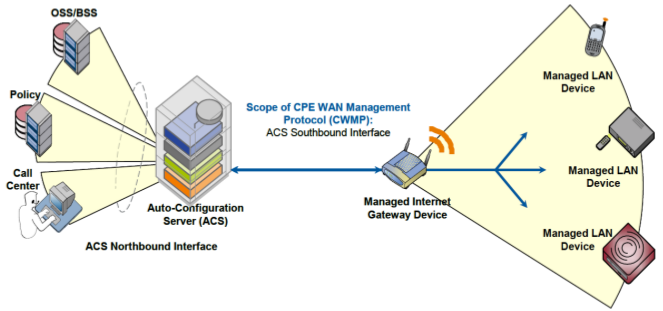
\includegraphics[scale=0.7]{./img/DM-TR-069-screen.png}
    \caption{Réseau de Device Management, côté \gls{acs} et côté Client}
\end{figure}
\paragraph*{}
L’un des objectifs du Device Management, pour l’équipe \gls{care}, est d’apporter un service d’aide et de dépannage aux clients, tous en restant à distance. Dans le but de ne pas avoir à faire déplacer un technicien sur place, pour un problème qui peut être résolu à distance par l’exécution de scripts, lancement de test et analyse, correction de bug. Le rôle de l’équipe \gls{care}, est de concevoir l’intégration de ces outils qui pourront être utilisés à distance.
\paragraph*{}
La supervision et la maintenance du parc Orange sont d’autres activités dans le
périmètre de l’activité du Device Management. Ce parc contient les différents produits
vendus par Orange et qu’Orange s’engage à maintenir. On comprend alors l’importance des
activités de supervision et de maintenance. Pour gérer ce parc, Orange a besoin, entre
autres, d’identifier les différents équipements présents et d’accéder à leurs  caractéristiques. Les outils de Device Management développés au sein de l’équipe \gls{care} permettent, cette fois, de remonter aux \gls{acs} toutes les informations nécessaires pour superviser et maintenir le parc. Il permet également de mettre à jour et corriger des bugs en envoyant de nouvelles versions de firmware aux équipements concernés. \\
\subsubsection{La norme TR-069}
\subsection{Objectifs envisagés}
\subsubsection{Première année}
\subsubsection{Deuxième année}
\subsubsection{Troisième année}

\section{Monté en compétence sur le protocole CWMP}
\subsection{Création d'un ACS Servlet}
\subsection{Études d'équipements}
\subsubsection{Présentation du réseau isolé}
\subsubsection{Test DNS}
\subsubsection{Test de comportement TR-069 d'équipement}
\subsection{Étude de client CWMP}
\subsubsection{Client EasyCWMP}
\subsubsection{Client tr69agent d'Orange}
\subsubsection{Résultats} %conséquence : création du toolkit !
\subsection{Impact sur mon parcours}

\section{Projet principal: Conception et développement d'un outil de test}
\subsection{Contexte}
\subsection{Présentation}
\subsection{Méthode de projet}
\subsection{Travail de préparation}
\subsubsection{Recherche de solution technique}
\subsubsection{Analyse de faisabilité}
\subsection{Conception}
\subsection{Réalisation}
\subsubsection{Travail en équipe}
\subsubsection{Développement}
\subsection{Déploiement}
\subsubsection{Environement}
\subsection{Communication et utilisateur}
\subsection{Livrable du projet}
\subsection{Difficultés, solutions et compétences acquises}
\subsection{Bilan et apport personnel du projet}

\section{Transfert de compétences}

\section{Bilan de compétences}

\section{Conclusion}
\subsection{Atteintes des objectifs}
\subsection{Progression}
\subsection{Synthèse de parcours}

\end{document}
